% Most of these belong in a .cls file

\documentclass[pdftex,12pt,a4paper]{report}

\usepackage[pdftex]{graphicx}
\usepackage{fancyhdr}
\usepackage[colorlinks=true,linkcolor={black}]{hyperref}
\usepackage{amsmath, amsthm, amssymb}
\usepackage{indentfirst}
\usepackage{multirow}
\usepackage{todonotes}
\usepackage[english]{babel}
\usepackage[utf8]{inputenc}
\usepackage{listings}
\usepackage{color}

\lstset{ %
  basicstyle=\footnotesize\ttfamily,  % the size of the fonts that are used for the code
  numberstyle=\tiny
  numbersep=5pt,
  tabsize=2,
  extendedchars=true,
  breaklines=true,
  keywordstyle=\color{red},
  stringstyle=\color{white}\ttfamily,
  showspaces=false,
  showtabs=false,
  xleftmargin=17pt,
  framexleftmargin=17pt,
  framexrightmargin=5pt,
  framexbottommargin=4pt,
  showstringspaces=false,
}

\usepackage{caption}
\DeclareCaptionFont{white}{\color{white}}
\DeclareCaptionFormat{listing}{\colorbox[cmyk]{0.43, 0.35, 0.35, 0.01}{\parbox{\textwidth}{\hspace{15pt}#1#2#3}}}
\captionsetup[lstlisting]{format=listing,labelfont=white,textfont=white,singlelinecheck=false}

\pagestyle{fancy}

\newcommand{\HRule}{\rule{\linewidth}{0.5mm}}

\setlength{\headheight}{15pt}

\begin{document}

\pagenumbering{roman}

\begin{titlepage}

\begin{center}

\textsc{\LARGE Master thesis draft}\\[1.5cm]

\HRule \\[0.4cm]	
{ \huge \bfseries Memory profiling techniques}\\[0.4cm]
\HRule \\[1.5cm]


\includegraphics[width=0.6\textwidth]{src/img/LinkUniv_staende}

\vspace*{1cm}

\begin{minipage}{0.4\textwidth}
\begin{flushleft} \large
\emph{Author:}\\
Andrei \textsc{Faur}\\
\end{flushleft}
\end{minipage}
\begin{minipage}{0.4\textwidth}
\begin{flushright} \large
\emph{LiU-ID:}\\
andfa683\\
\end{flushright}
\end{minipage}

\vfill

{\large \today}

\end{center}

\end{titlepage}


\vfill

\addcontentsline{toc}{chapter}{Acknowledgements}
\thispagestyle{empty}

\begin{center}
Give credit where credit is due
\end{center}

\vfill


\par\vfill

\chapter*{Abstract}
\addcontentsline{toc}{chapter}{Abstract}

The abstract is, for now, quite abstract.

\par\vfill\null


\input{src/base/contents}

\lhead{\bfseries Master thesis draft - Andrei Faur}
\chead{}
\rhead{\thepage}
\lfoot{}
\cfoot{}
\rfoot{}
\renewcommand{\headrulewidth}{0.4pt}

\pagenumbering{arabic}

\chapter{Introduction}
\label{chapter:intro}

\textbf{So it begins...}\\

\newpage

\textbf{And so it continues...}\\

\textbf{Det funkar på svenska också! öåöäöåöäöåä}\\

\chapter{Memory Management Concepts}
\label{chapter:memmgmt}

Throughout the lifetime of a process its memory requirements change. Whether the process has to create more objects or allocate arrays or even temporary variables, it has to have a way of requesting more memory and a way to release that memory when it is no longer needed. Since our purpose is to actively monitor the exact memory consumption of a process\footnote{For simplicity, let us assume that the piece of software we are interested in monitoring runs only in one process.}, the underlying mechanisms of memory allocation and deallocation are of direct interest.  This chapter explains these mechanisms and explains how each of them are relevant to our original goals of finding out how much memory a process consumes and how different parts of that process interact with each other to reach that specific memory consumption state. The terms described in this chapter will be used throughout the rest of the thesis and they constitute the framework of our problem.

\newpage

\section{Virtual Memory}
\label{section:virtmem}

Virtual memory is a mechanism used by modern operating systems in order to give processes the illusion that there exists only one type of memory in the system which exhibits the behaviour of a directly addressable read/write memory. In addition, most operating systems run processes in separate address spaces providing the impression that processes have exclusive access to the virtual memory\footnote{There exist operating systems which use a single global address space, such as OS/VS1 and IBM i, but they still include mechanisms by which processes are stopped from accessing each other's addresses}. This is accomplished by the operating system by avoiding the direct use of physical addresses and instead making processes use logical addresses which then get translated by the operating system and the memory management unit into physical addresses. Figure \ref{fig:virtmem} shows a 32-bit system with two processes and their address spaces and the way they are mapped to physical memory and other devices.

\begin{figure}[htb]
\centering
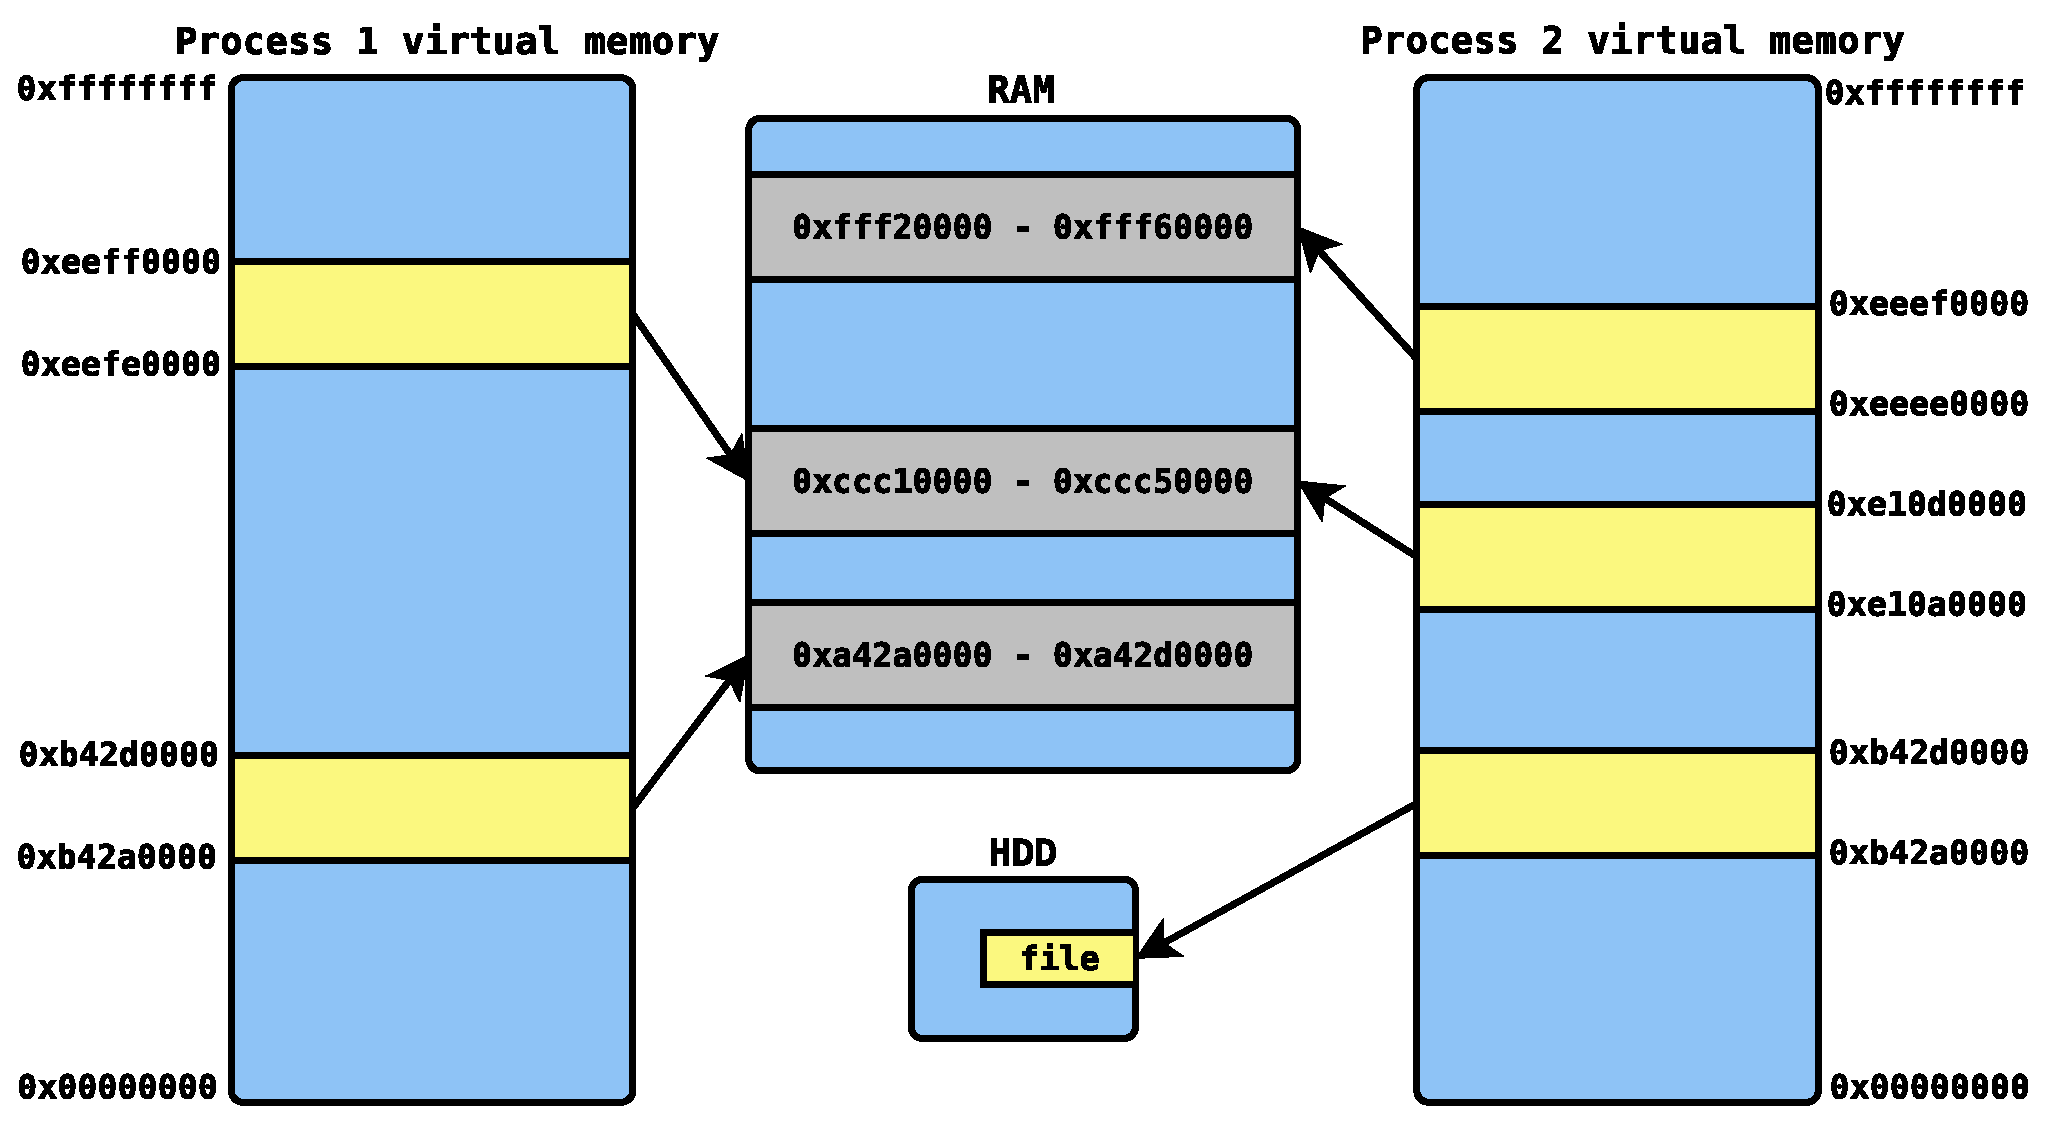
\includegraphics[width=0.8\textwidth]{src/img/virtmem}
\caption{Two processes mapping memory in diverse ways}
\label{fig:virtmem}
\end{figure}

Note that the virtual memory mechanism allows different process to share memory between each other by mapping the exact area of physical memory into possibly different areas of virtual memory and also map other devices into their address space, including files from the disk. The same virtual address in different processes can be mapped to different places, enforcing the idea of address space separation. The exact mechanisms which make virtual memory work and concepts such as translation lookaside buffer, paging, multi-level page tables, page replacement algorithms have been described in great detail in OS literature such as \cite{Silberschatz08}, \cite{Tanenbaum07}, \cite{Drepper07} and many more and since these exact details do not have an impact on our analysis, the reader is referred to these for more in-depth knowledge.

Monitoring a process's memory thus becomes a problem of monitoring the way its virtual memory is mapped. This leads to the question of determining which area of a process's virtual memory we are interested in monitoring. Do we monitor all of it or just specific parts? In order to answer that question we first have to understand exactly how a process's virtual memory is organized.

\section{Memory Layout}
\label{section:memlayout}

In order for a program to become a process it has to be loaded into memory\footnote{In systems with virtual memory no bytes of the program are actually copied into main memory but rather a part of the newly created process's address space is marked as containing the code. Only when the code will be executed will it be brought into main memory.} by a part of the operating system called the loader. The question is then how is the process's virtual address space organised? Several formats have existed over the years, such as Unix's a.out, MS-DOS's COM and the more recent ELF format. While these might differ drastically in terms of the object code representation, ultimately their goal is to produce a memory layout similar to Figure \ref{fig:virtmemlayout}.

\begin{figure}[htb]
\centering
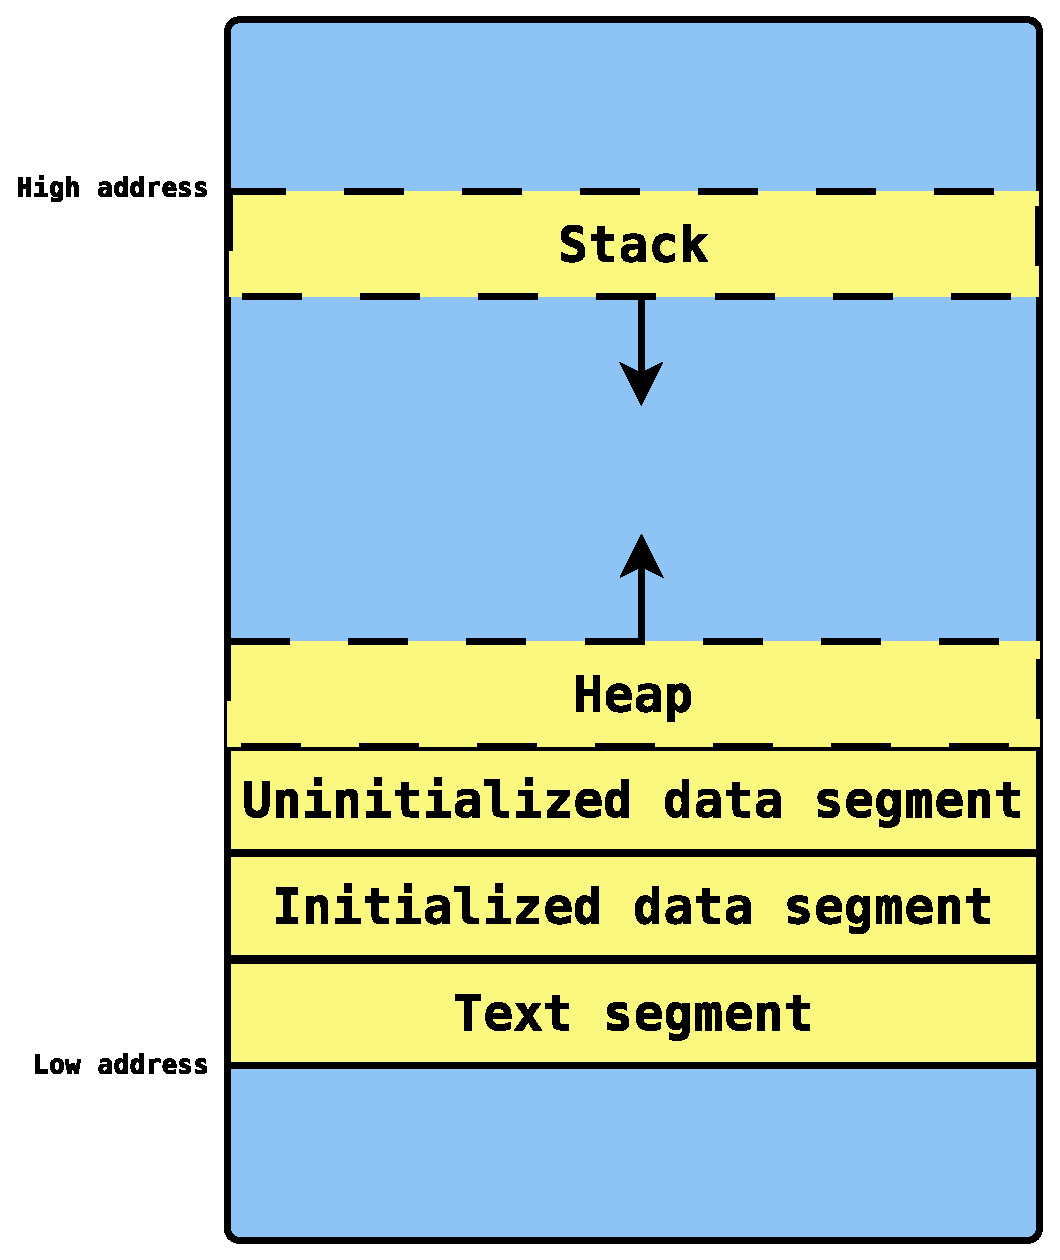
\includegraphics[width=0.4\textwidth]{src/img/virtmemlayout}
\caption{Typical virtual memory layout}
\label{fig:virtmemlayout}
\end{figure}

The segments represented are:
\begin{itemize}
\item text segment - which contains the actual code
\item initialized data segment - global variables which are initialized by the programmer
\item uninitialized data segment - variables in this segment are initialized to 0 or NULL before the program begins to execute
\item the heap - used for allocating more memory during runtime, described in section Y
\item the stack - used for function calls, as described in section X
\end{itemize}

The text segment and static data segments (initialized and uninitialized) usually do not change in size during the lifetime of a process so they are of little interest; their size can be determined from compile time and can be reported easily. The stack and the heap, which usually grow towards each other, are constantly changing but their purpose is different. They will both help us in reaching our goal and, as it will be seen in the next subchapters, ultimately we will be interested in monitoring the heap, using the stack just as a source of additional data.

\section{The heap}
\label{section:heap}

The heap is where all dynamic allocations\footnote{Note that there exist system calls such as \textit{alloca} which allow dynamic allocation of space on the stack. These are rarely used and as such they won't be taken into consideration} done during the lifetime of a process are stored. Operating systems offer system calls which expand the heap, thus providing access to more memory. For example, Linux offers the \textit{brk} and \textit{sbrk} system calls which change the location of the end of the process's data segment, while Windows has the \textit{*Alloc} system calls. It is however rare for high level applications to call these routines directly; instead, they use external libraries or libraries provided by the language they are written in. For example, the classical ways of allocating memory in UNIX systems makes use of the following standard C library calls:

\begin{itemize}
\item \textit{malloc/calloc} - allocates a number of bytes from the heap and return a pointer to the beginning of the block; calloc initializes this region to zero
\item \textit{realloc} - given a pointer to a previously allocated block, expand that block by a given size; it is not guaranteed that the resulting block lies in the exact place on the heap since there might not be enough contiguous space after the block
\item \textit{free} - given a pointer to a previously allocated block, release that block and mark the memory as free
\end{itemize}

Programs written in C++, even though able to call the above routines, make use of the \textit{new} and \textit{delete} operators. These operators however, in the standard C++ library, ultimately translate into calls to the above.

An additional system call available in Linux for mapping memory is \textit{mmap} which is more flexible than \textit{brk}. It allows mapping of any region of the virtual memory not only to RAM, but to files too. Given how everything in Linux is modeled as a file, including devices, mmap can basically map virtual memory to any device's internal memory as long as the latter allows it. The \textit{munmap} system call does the reverse process of unmapping virtual memory.

It is clear now that in order to monitor a process's memory consumption we have to either hook the above calls or provide wrappers around them. By doing either of these we can answer our original question of how much memory an allocation site is requesting. By allocation site we refer to a point in a program where one of the above routines/operators is invoked.

Another interesting point worth mentioning is the problem of which area of virtual memory will be selected for mapping when one of the above routines is called. It is the job of the memory allocator to selected the locations in such a way as to minimize fragmentation, maximize cache locality and provide fast allocation and deallocation speed at the same time\cite{Wilson95}. These goals sometimes clash and trade-offs have to be made. Techniques such as reference counting, pooling and garbage collection are sometimes used in conjunction with allocators in order to lessen the burden of memory management from the programmer\cite{Detlefs94}. All of these have to be taken into consideration in order to do correct memory profiling. Communication with the garbage collector, for example, might be the only way to detect when memory gets deallocated since memory is no longer explicitly released. Another example could be allocators which preallocate memory in advance so that subsequent memory allocation requests are faster. In this case we have to ask ourselves if we are interested in every mapped byte from virtual memory or just those bytes which can be potentially accessed?

Memory allocators use different techniques for selecting which memory region to map when an allocation is requested, such as:
\begin{itemize}
\item \textit{Memory pooling} - one or several chunks of the address space are requested by the allocator in advance. Subsequent allocation requests will be given chunks from these pools, thus avoiding unnecessary system calls. Different pools might have different purposes such as one targeted towards small allocations while the others are structured in such a way as to minimize fragmentation. The advantage with pools is that they can usually be cleared using a single call and some implementations even allow their creation and destruction at will. This takes some of the burden of memory management from the programmer. Keeping track of every allocation is no longer necessary since a pool can be destroyed by just a simple call and all previous allocations made from that pool are instantly gone.
\item \textit{The buddy system} - this technique divides the address space into blocks which have the size multiple of powers of two. The initial size of these blocks and their minimum size is usually platform dependant and also chosen empirically, based on most common allocation sizes. When an allocation is made, of size smaller than the smallest block available, one of these blocks is chosen and then divided in two. The process is repeated until the division would lead to the creation of blocks of smaller size than the allocation requested. One of the blocks thus created is then given to the allocation. The name of this techniques comes from what happens when a block is freed. All the previous divisions created "buddy blocks" of equal sizes. When one of these blocks is freed then its buddy is checked to see if it is free. If it is, then the two are joined into a larger block and the process repeats.
\end{itemize}

One thing that most allocators have in common is that they need a way of keeping track which parts of the memory have been allocated. For example, in the buddy system, either linked lists or trees can be used to store blocks which have the same size. When memory pooling is used, there is both a need of keeping track of all the pools available and keeping track of how each pool is organized. A simple allocator might just use two lists: one keeping track of all the available chunks of memory and their sizes and one for those which are taken. One thing which is clear is that all this bookkeeping does incur overhead both in time and in the used memory. More than that, for correct memory profiling, close communication with these allocators might be required in order to see how memory is allocated.

\section{The stack}
\label{section:stack}

The stack is used by processes to keep track of the call chain. Each time a function is called a new stack frame is created and pushed on the stack. Upon return from that function, the stack frame is popped. A stack frame's exact structure is dependant on the platform on which the code is running, but in all cases they at least contain the following:

\begin{itemize}
\item the arguments passed to the function
\item the return address back to the caller's code
\item space for the function's local variables
\item space for the function's temporary variables in case they can not be stored in registers
\end{itemize}

\begin{figure}[htb]
\centering
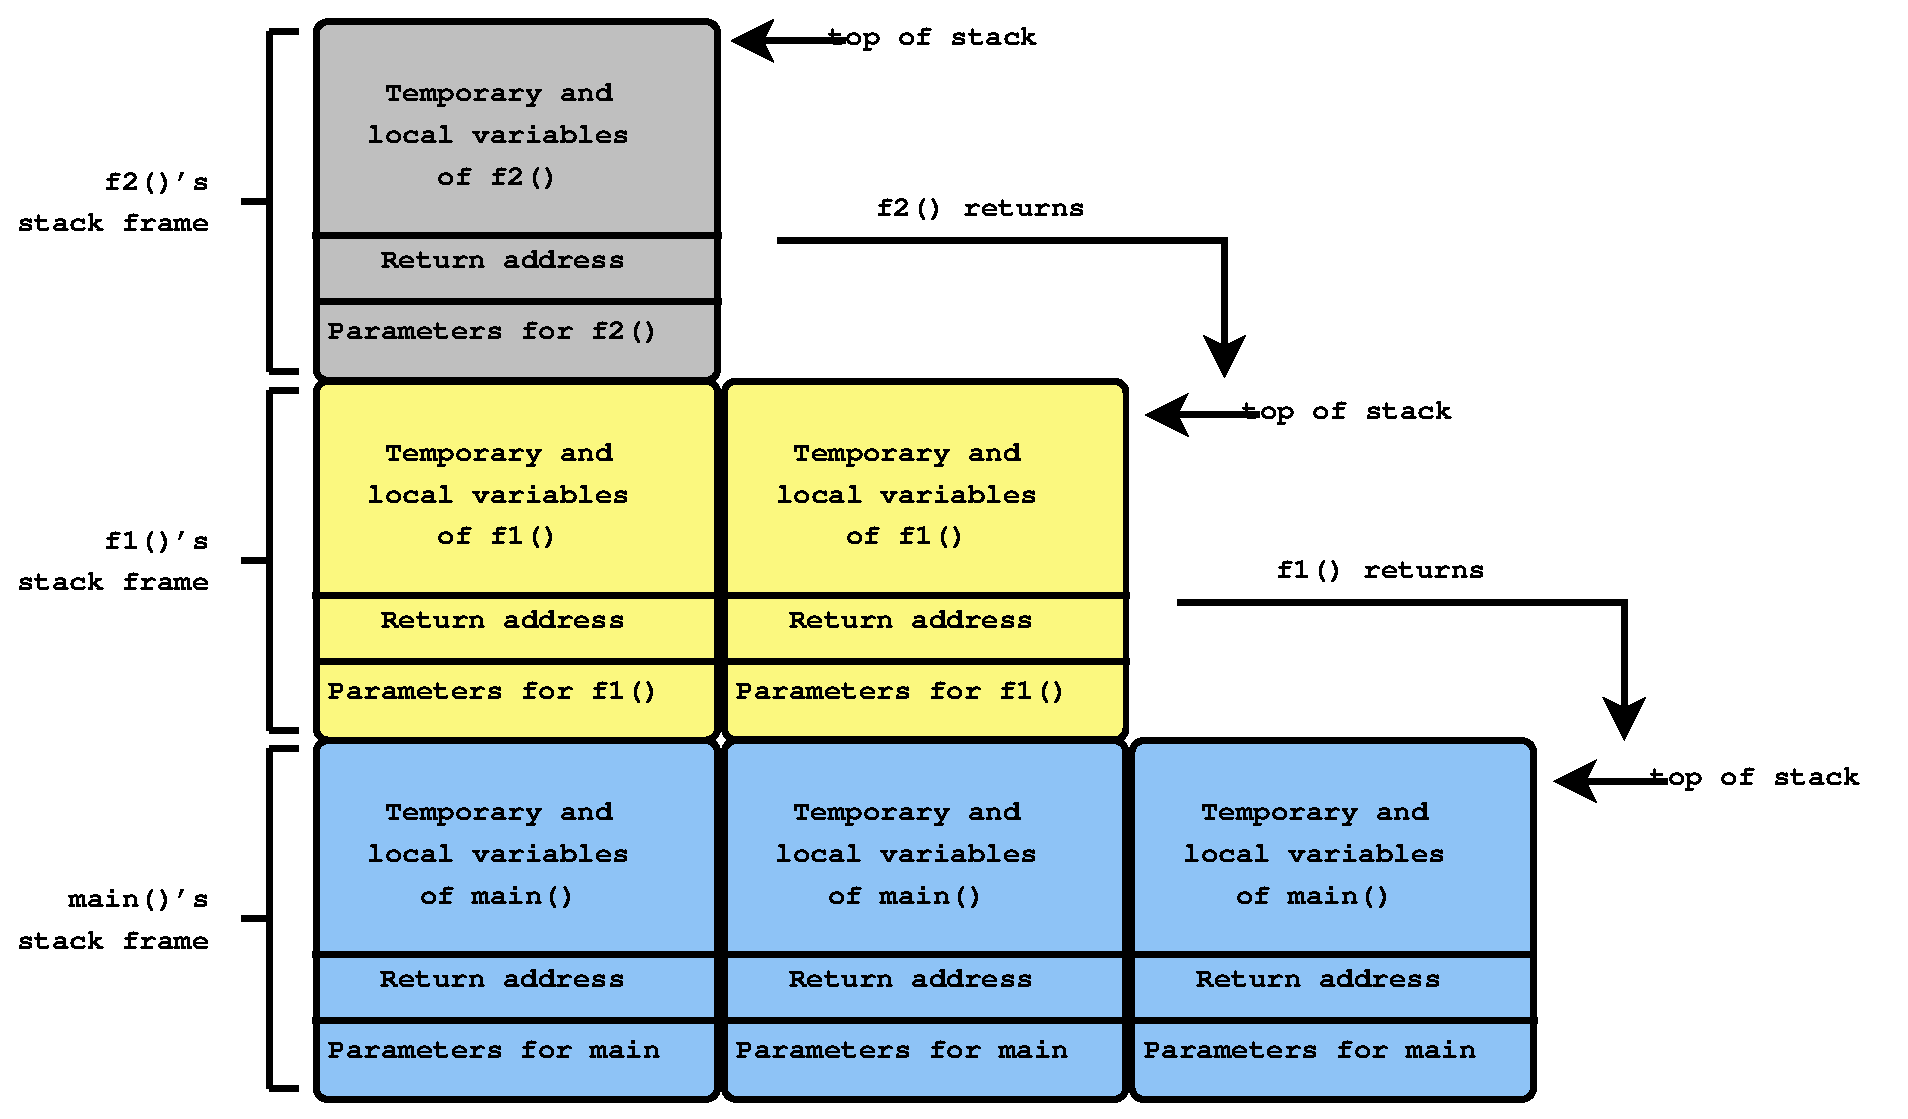
\includegraphics[width=0.8\textwidth]{src/img/stacklayout}
\caption{Typical stack layout}
\label{fig:stacklayout}
\end{figure}

Let us assume we have a process whose current call chain is main()-f1()-f2(). The process's stack and its evolution follow something similar to Figure \ref{fig:stacklayout}.

The information contained in the stack at any point in time allows us to trace the call chain from the current execution point all the way to a program's entry point. Suppose that f2() in Figure \ref{fig:stacklayout} did an allocation in which we were interested. By using the stack, we are able to go back from an allocation site through as many callers as we want. This answers one of our original questions: who is responsible for allocating memory?

\todo{dsa.pdf - Dynamic storage allocation}
\todo{spe895.pdf - Memory allocation costs in C and C++}
\todo{jemalloc.pdf - jemalloc description}

%\chapter{Memory profiling techniques and tools}
\label{chapter:instrmet}

\textbf{And so it continues...}\\


%\chapter{A hybrid memory profiling approach}
\label{chapter:hybrid}

\textbf{And so it continues...}\\

\chapter{Methods}
\label{chapter:methods}

In this chapter we will focus on the description of methods used in obtaining dynamic memory allocation information. We will start by presenting approaches used by profilers in general and see how these are applicable to memory profiling in particular. Given the fact that we are concerned in both the size and the locations of memory allocations and since these two involve different approaches, we will present different methods of obtaining relevant information separately for these two. Finally, a test program and the platform on which it was run will be described, upon which all these methods will be tested. This will provide a good performance reference in order to determine the overhead the memory profiling techniques induce.

\section{Profiling methods}
\label{section:profilingmethods}

Profiling definition.

In this section we will describe the most common techniques used for profiling today. Some of these techniques do not target memory profiling specifically, but nevertheless they can be used for this purpose.

Types of profiling + short description for each.

mprof.pdf [Memory allocation profiler for C and LISP]

p28-kumar.pdf [Low overhead program monitoring and Profiling]

science.pdf [Efficient dynamic program monitoring on multi-core systems]

zhao-cgo07-umi.pdf [Ubiquitous memory introspection]

10.1.1.104.4146.pdf [Dise: A Programmable Macro Engine for Customizing Applications]

shetty\_ibmpac04.pdf [HeapMon: memory bug detector]

WRL-94-2.pdf [ATOM, system for implementing customized program analysis tools]

paper.pdf [gprof - a call graph execution profiler]

wenke.pdf [Framework for instruction-level tracing and analysis of program executions]

dynamopldi.pdf [Dynamo optimization system]

10.1.1.90.5250 [Optimally profiling and tracing programs]

Continuous profiling: where have all the cycles gone (paywalled, have to check liu online library)
System support for automatic profiling and optimizatins: paywalled

\subsection{Code instrumentation}
\label{subsection:codeinstrumentation}

Definition of instrumentation in general.

Types of instrumentation + description for each of them.

Give examples of tools and how they work.

valgrind2007.pdf [How Valgrind works]

shadow-memory.pdf [How to shadow every byte of memory]

a5-venkataramani.pdf [MemTracker, tool based on PIN]

interact-9\_IEEE\_23210082 [Automatic Low overhead instrumentation using the LOPI Framework]

Tamches99FineGrained.pdf [Fine-grained dynamic instrumentation of kernels]

apiPreprint.pdf [An API for Runtime Code Patching]

phd2004.pdf [Nethercote dynamic instrumentation phd]

derek-phd-thesis [Efficient, transparent, comprehensive runtime code manipulation]

dtrace\_usenix [Dynamic instrumentation of production systems]

10.1.1.85.4883 [PIN, building customized program analysis tools with dynamic instrumentation]

VEE2006.pdf [HDTrans, low-leve dynamic instrumentation system]

Reversible debugging using program instrumentation - paywalled

\subsection{Statistical profiling}
\label{subsection:statisticalprofiling}

Definition of statistical profiling.

How it works.

Examples of tools.

swat\_asplos\_final.pdf [Leak detection using statistical profiling]

dcs-tr-424.pdf [Reducing the cost of instrumented code]

\subsection{Performance counters}
\label{subsection:performancecounters}

What they are, how they are used. Examples from modern x86 architectures maybe. Oprofile et. al.

pap182.pdf [Memory profiling using hardware counters.]

papi-ugc2001.pdf [PAPI cross-platform interface to hardware performance counters]

\subsubsection{Hardware-assisted profiling}
\label{subsubsection:hardwareassistedprofiling}

Not the same as performance counters. This one actually uses dedicated hardware to monitor different stuff rather than simple counters.

venkataramani\_hpca07.pdf [hardware for memory access monitoring and debugging]

LBA\_ISCA08.pdf [Flexible Hardware Acceleration for Instruction-Grain Program Monitoring]

LBA\_asid2006.pdf [Log-Based architectures for general-purpose monitoring of deployed code]

tacodec04.pdf [Architectural support for dynamic monitoring]

profiler.hpca.pdf [A programmable co-processor for profiling]

\subsection{Event-based profiling}
\label{subsection:eventbasedprofiling}

Events are triggered either through software or hardware exceptions. Give examples of how these might be used.

\section{Heap profiling}
\label{section:heapprofiling}

In section \ref{section:memlayout} we have presented the typical layout of a program after it has been loaded into memory. While in modern programs there exist a lot more sections than the ones described, the heap is usually the one where most of the allocations are done. Thus, we will not concern ourselves with the other sections because their size is pre-determined from compile time and they do not suffer modifications during run-time. In this subchapter we will present different methods of determining the size and the point in the program where allocations on the heap are performed.

\subsection{Allocation size profiling}
\label{subsubsection:allocationsizeprofiling}

The first problem we want to solve is the problem of determining the total size of all the data that exists on the heap. More specifically, we want to be able to answer one of our original questions: how much memory have the classes/modules allocated on the heap?

\subsubsection{Overloading memory allocation routines}
\label{subsubsection:overridingroutines}

A first solution to keeping track of all the allocations that a program has done is to overload the routines that do the allocations. By doing this, we can insert our own code in the routines, code which allows us to manipulate the allocation information in any way we want. The routines which have to be overloaded are the same ones presented in section \ref{section:heap}.

There are several problems with this approach, one of them related to the actual implementation of the mechanism. Overloading the routines means replacing them with our own while keeping the functionality intact. This has to be done in a way that is transparent to the running program and has very little overhead, preferably none. Different approaches exist:
\begin{itemize}
\item The \textit{new} and \textit{delete} operators can be overridden globally through language constructs provided by C++ itself. By looking at the way these two operators are implemented in the standard C++ library, one could provide an implementation that is identical but also provides additional profiling code.
\item For the \textit{malloc}, \textit{realloc} and \textit{free} routines, GCC provides hooks which allows their behaviour to be modified. These hooks are actually variables declared in malloc.h : \_\_malloc\_hook, \_\_realloc\_hook, \_\_free\_hook, \_\_memalign\_hook. All of these can point to independent routines which are called whenever the original allocation routines are called. These routines' signature contains a caller parameter which is the return address found on the stack when the allocation routines were called, thus allowing allocation point tracking\cite{GCCman}. The downside with using this method is that it is GCC specific, so if other compilers are used then either a similar mechanism has to exist for them or this approach does not work.
\item A separate library providing implementations for all the C-level allocation routines can be used. Since \textit{new} and \textit{delete} are also using these, they will also be taken into account, thus covering the whole range. This library can then be linked with the original program in such a way that the overloaded routines are used instead of the ones provided by the standard library. This is the approach that Valgrind uses, by exporting symbols which take precedence over the ones in glibc.so\cite{Seward02}. While it does have the benefit of being unintrusive it still is dependant on the build system, especially on the linker used.
\item Another solution is to provide wrappers for the allocation routines, which will be used instead of the original ones. The downside to this is that it is very intrusive since all of the original calls have to be replaced with calls to the wrappers. Tools that do this replacement automatically can be used.
\end{itemize}

Hunt and Brubacher\cite{Hunt99} classify techniques of intercepting function calls on Windows into four categories:
\begin{itemize}
\item \textit{Call replacement in application source code} - All of the above, except for the one involving providing a separate library fit into this category.
\item \textit{Call replacement in application binary code} - By using symbolic information call sites are identified and jump code to profiling routines can be inserted
\item \textit{DLL redirection} - Similar to using a separate library, the internals of this technique are Windows-specific
\item \textit{Breakpoint trapping} - By inserting a debugging breakpoint in the function we wish to intercept, we can have the debug exception handler reroute to a profiling routine. This involves a separate process (the Windows debugger) and it has the downside of suspending all application threads.
\end{itemize}
More than that, they compare these techniques with their interception implementation and show that the overhead varies from 250ns to 400ns with call replacement and DLL redirection, while breakpoint trapping has an overhead on the order of microseconds. If we add to this the fact that the profiling routine itself induces overhead, along with the fact that it proves to be not-trivial to implement and sometimes even intrusive, we can conclude that overloading the memory allocation routines in order to obtain live heap information is not a viable solution.

\subsubsection{On-demand memory tracking}
\label{subsubsection:ondemandtracking}

We now take a different approach to keeping track of the amount of allocated memory, one which does not involve interfering with the allocation routines. To do that, we note that most of the data living on the heap is structured in some way. Whether it is stored in just a simple array of integers or more complex data structures, it has references to it which can be accessed to determine its size. The advantage of such an approach is that we control when the size is determined and thus implicitly control when the overhead of this computation is imposed. The idea is to trigger the computation of the data structure's size on-demand, shifting the constant overhead of overloading memory allocation routines to a one-shot significantly larger overhead which could potentially be triggered during a period of low processor utilization.

The first possible way of keeping track of a data structure's size is \textit{counter-based}. This is as simple as keeping a variable which keeps track of the size that the data structure occupies, counter which is updated accordingly for each modification of said data structure. For example, an addNode function for a linked list would increment the variable with the size of the newly added node, while a removeNode function would decrement it in a similar manner. Naturally, more complex structures would require perhaps more counters and an even more careful accounting method, but the idea is the same: have a set of variables which accurately represent the size of the data structure at any point in time. The biggest advantage of this method is that it has very low overhead. The bulk of the accounting is spread between the methods which update the data structure and usually this involves only incrementing or decrementing the variables. When the information related to the data structure's size is required on-demand, all there is to do is to return the variables which contain this information, making this approach very lightweight in terms of overhead. The downsides are that it is intrusive, but, more importantly, it is very hard to maintain. Experience has shown \cite{Nethercote12} that people forget to update the profiling code when the data structure is updated, or partially update the profiling code since it is spread out in many methods that have an impact on the data structure. This leads to incorrect reporters that might not even be acknowledged as incorrect until after some serious debugging.

Since the main problem with the above method was that the profiling was spread in so many places that it was hard to keep track of all of them when they needed to be updated, perhaps there is a way to aggregate all of the profiling into one place. This is the idea with \textit{traversal-based} profiling. Have one method (or several, if multiple statistics are monitored) which traverses the data structure and reports its size. This does have significantly larger overhead than the above technique, especially if the data structure is large, but it is easier to maintain. Also, let's not forget that the idea is to trigger this traversal on-demand. There are several complicating factors with this approach, such as:
\begin{itemize}
\item Cycles in the data structure could lead to the same memory being counted twice
\item When using inheritance, the sub-classes must make sure not to take into account the memory of their parents again
\item Complex structures require complex traversals which are not trivial to implement and therefore might be difficult to maintain too
\end{itemize}

Note that by using these methods we have now lost the ability to detect memory leaks. If we would have kept track of every allocation then this extension would have been possible with some effort. However, this was never the purpose of this thesis so memory leak detection is out of scope. Allocations which are done and then never freed and do not have a reference to them will still continue to live on the heap and will occupy space but will not be detected by the profiler. This is considered a programmer error and specialized tools for their detection do exist.

In conclusion, both of the above methods are highly intrusive, requiring access to the source code. Counter-based profiling is the lightest of the two, but the hardest to maintain, while traversal-based has a higher overhead but better maintainability. Which one should be chosen is a matter of the project's size and priorities.

\subsection{Allocation point profiling}
\label{subsection:allocationpointprofiling}

The second problem we want to solve is to be able to answer two of our initial questions: who did the allocation and what lead to the allocation being done? The answer to both of these questions is found in the stack trace from the moment the allocation is done.

\subsubsection{Manual stack traversal}
\label{subsubsection:manualstacktraversal}

As we have seen in section \ref{section:stack}, the stack is where we can find information about the call chain that led to an allocation. Accessing the stack is, unfortunately, not a straight forward endeavour, mostly because each platform has subtle differences in the way the stack is implemented, which makes accessing it a bit difficult. Some compilers provide already implemented routines which hide away the details of the underlying architecture. One such example is GCC, which provides the \textit{backtrace} function. This function returns the call chain in a buffer of a given size. What it actually does behind the scenes is perform a stack walk.

A piece of software which does not want to be tied to a specific compiler should not use such compiler-provided functions but instead opt to implement its own. To give an idea of the complexity of a stack walker we now present the C implementation of such a program on an x86 Linux platform.

Keeping in mind the structure of a stack frame, described in section \ref{section:stack}, we need to determine two things:
\begin{itemize}
\item how to jump from stack frame to stack frame
\item how to obtain the return address from each frame, knowing that this return address is what determines the caller
\end{itemize}

Knowing only the beginning of the stack is of no use to us since we do not know how much local data has been pushed on the stack and therefore cannot determine precisely where the return address is. In this case, we can use the ebp register which is commonly used to point at the beginning of the current local data. However, we know that just above the local data lie the ebp value of the caller and the return address. Thus, to jump from stack frame to stack frame we have to follow the ebp values and to get the return address we just look at the value above the ebp on the stack.

Without going into the exact implementation details, a solution that does this is shown in \ref{stackwalker}:
\begin{lstlisting}[label=stackwalker,caption=Simple stack walker for x86]

struct frame {
        struct frame* old_fp;
        long ip;
};

struct frame *frame, *fp;

asm("movl %%ebp, %0" : "=r"(frame));

fp = frame;

for(; !(fp < frame) && !(fp < stack_bottom));
      fp = (struct frame *)((long)fp->old_fp))
   {
       // Do something with the return address from fp->ip
   }
\end{lstlisting}

The end result is that we can obtain a list of return addresses which can then be further used to obtain the actual names of the routines forming the call chain. Inserting the above routine in every allocation point would give us a stack trace which can be used to determine the exact call chain leading to the allocation.

There are, however, several downsides to this approach. First of all it is heavily platform dependant. The above code only runs on x86, using specific GCC directives. Not only that, but it relies on the fact that the code has been compiled with frame pointers activated. Some compiler-level optimizations remove the frame pointers to reduce stack frame size and obtain a small increase in speed. Different hardware platform may have a completely different stack frame format so the code would have to be rewritten for each compiler/platform combination, leading to something that would probably be very hard to maintain. The second problem is overhead. Attaching this code to every allocation point can lead to unnecessary overhead especially if we are not interested in the associated stack traces. A better method would be to activate the stack tracing on-demand, just for those allocations in which we are interested.

\subsubsection{Low overhead tracepoints}
\label{subsubsection:lowoverheadtracepoints}

The problem of low overhead tracepoints has been under discussion for a long time, especially in the context of debugging. The DTrace tool for Solaris allows probes to be inserted into a running program which have low overhead when they are disabled\cite{Cantrill04}. Such implementations have also been attempted on SPARC\cite{Kessler90} and the LTTng project had a series of tools dedicated to tracing Linux both in userspace and kernel\cite{Desnoyers09}. We will present the approach currently taken by the Linux kernel in this section.

A naive implementation of an on-demand triggerable tracepoint would just check the truth value of a flag and, based on that value, either call the tracing routine or not. It could be something as simple as the code in \ref{tracepoint0}. There are some problems which stem from this such as the need of a data structure which keeps a list of all the available tracepoints and implements some naming scheme allowing the user to enable/disable them independently. The question is if there is some way to avoid the condition check so that a disabled tracepoint would have even lower overhead.
\begin{lstlisting}[label=tracepoint0,caption=Naive tracepoint implementation]
...
if (tracepoint_enabled)
	trace();
...
\end{lstlisting}

The idea is to keep a list of all the statically defined tracepoints. In our case, since we want all allocation points to be traceable, there will be a tracepoint for each of them. This list is built by the compiler during compilation and placed in a special section in the executable which can be accessed during runtime. At the same time, tracepoints which are disabled are replaced with nop operations. To activate a tracepoint during runtime one has to lookup its address in the tracepoint table and replace the nop instruction from that address with a jump to the place in the code which calls the tracing function. The key to having this work is special compiler support for moving code which can be jumped to, but not accessed directly, out of line\cite{GCCasmgoto}. The listing from \ref{tracepoint1} shows the way this is done in the Linux kernel, along with a typical usage scenario.
\begin{lstlisting}[label=tracepoint1,caption=Linux kernel jump label implementation]
static __always_inline bool static_branch(struct jump_label_key *key)
{
        asm goto("0: nop\n\t"
                 ".pushsection __jump_table, \"aw\" \n\t"
                 ".balign 4 \n\t"
                 ".long 0b, %l[l_yes], %c0 \n\t"
                 ".popsection \n\t"
                 : : "i" (key) : : l_yes);
        return false;
l_yes:
        return true;
}

#define TRACE(name)
        static const char
        __tpname_##name[]
        __attribute__((section("__tracepoints_strings"))) =
                #name;

        static struct tracepoint
        __tracepoint_##name
        __attribute__((section("__tracepoints"))) =
                { 0, __tpname_##name, { 0 } };

        static struct tracepoint * const
        __tracepoint_ptr_##name
        __attribute__((section("__tracepoints_ptrs"))) =
                &__tracepoint_##name;

        if (static_branch(&__tracepoint_##name.key))
                trace(&__tracepoint_##name);
\end{lstlisting}

It works by inserting a nop at the label defined by \textit{0:}. In the section called \textit{\_\_jump\_table} we save the address of that label, the address of the label to jump to when the tracepoint is activated, along with a key identifying the tracepoint uniquely. Since the routine is typically used in a branch, and since it will always evaluate to false, a compiler will want to remove the code completely since it is unreachable. However, due to the jump to the \textit{l\_yes} label, it is not removed completely but moved somewhere out of line thus leaving only the nop instruction in place. We know where the code is moved because we have saved the address of the \textit{l\_yes} label, thus, in order to activate the tracepoint we have to replace the nop with a jump to that address.

This implementation shows that it is possible to achieve a tracepoint implementation whose only significant overhead is related to the code size of the nops and the out of line code. The downside is the same as the stack walker's: the implementation is platform specific. In this case it might even be worse since the optimization that the GCC compiler does by moving the code out of line and allowing labels inside an assembly block might not even be possible in other compilers. Permission to modify the program's code during runtime is also required and this might not be allowed in secure environments. The main issue is thus one of maintainability and of deciding if the cost of implementing and maintaining such a solution is indeed lower than the benefit of being able to trace call chains in key points of the program.

One final note to keep in mind is that the question we are asking is if it is possible to implement the above and tie it into a piece of software so that it can be used live and without damaging its performance. There are tools which already do this sort of tracing, such as DTrace mentioned above and even Valgrind so it is not an issue of implementation but rather performance and maintainability.

\subsubsection{Global stack object}
\label{subsubsection:globalstackobject}

The above two solutions suffer most on the maintainability side because of their platform dependencies. The question which naturally follows is if we can abstract away those parts into something which is independent of the platform we are running on. The answer to this would be to keep our own pseudo-stack (or stacks in case of multiple threads) which is globally accessible and can be queried regarding its state at any time. We say pseudo-stack because we would only be keeping the function names in it since that is what we are interested in. To have this working, each function must call one routine at its entry point pushing its name on the stack and another at its exit point for popping. A tool which inserts these calls automatically can be created.

The global stack object thus removes the need of having a stack walker. However, invoking the object for providing the call chain still requires the tracepoints and making these platform independent leads us to the naive implementation from listing \ref{tracepoint0}.

\section{Test program description}
\label{section:testprogram}

\chapter{Results}
\label{chapter:results}

\section{Test infrastructure description}
\label{section:testprogram}

In order to create a test program for the above methods we have to determine the requirements for such a program. Since we are interested in determining allocation sizes and allocation points, the test program has to provide a sufficiently diverse combination of these. Our program also has to be deterministic so that we test the methods against the same sequence of allocations. The number of allocations has to be sufficiently high so that the overhead of monitoring becomes noticeable.

In order to keep things simple and focus on the techniques and not on what the program does, the main task of our test program is to allocate a linked list whose nodes contain pointers to malloc-allocated memory whose size is controllable. In other words, we have a list of memory regions allocated with malloc. The linked list's nodes are also heap allocated and since there is one node for each allocation we can say that the number of actual allocations is twice that we give as input to the program. We are also interested in being able to control the depth at which the allocations are made, in order to be able to determine the overhead of stack tracing as the stack increases in size.

Most programs have memory usage patterns containing a mix of allocations and deallocations. Having a test program which contains just allocations would not be representative for the majority of these patterns. Thus, we introduce the capability of deallocating some of the allocated memory through a simple counter which triggers the release of a previously allocated memory region. In the end, the core loop of the test program has the following pseudocode, where capitalized variables are given by the user:

\newpage

\begin{lstlisting}[label=pseudotest, caption=Test program core loop]
for NR_ITERATIONS do
	for size = START_SIZE, size < END_SIZE, size += STEP_SIZE
		call function such that allocation of size bytes is made at depth DEPTH in the call stack
		if DEALLOCATION_COUNTER reached zero then free previous allocation and reset DEALLOCATION_COUNTER
\end{lstlisting}

First, we want to determine the overhead of determining the size of each allocation and compare it with the overhead of periodically sampling and traversing data structures. These are the two major approaches we can take in determining the amount of memory a specific program occupies. The final goal of allocation size monitoring is to be able to determine memory consumption on a per-module basis. Total memory consumption is not an issue, as this can be determined through other mechanisms which are usually provided by the operating system. The main problem is to have more fine grained memory reporting. For now, however, the test program is only interested in determining the total size of all the allocations we do. At this point, we are only trying to determine the overhead of obtaining the allocation data so we ignore the overhead of its utilization in finely grained memory reporting. In order to do this, we test the following scenarios:
\begin{enumerate}
\item \textit{On-demand data structure traversal} - go through the linked list and use malloc\_usable\_size on each node and the memory region it points to
\item \textit{On-demand counter based monitoring} - have the linked list hold a counter representing the total allocated size, which is updated whenever a node is added or removed; access the counter whenever the total allocated size is required
\item \textit{GCC provided malloc hooks} - use these to insert own code which updates a global variable containing total allocated bytes
\item \textit{GCC aided call replacement} - write own allocation routines which do the counting and then call the existing ones to actually do the allocation
\item \textit{Manually defined malloc-wrappers} - use the preprocessor or just write own routines which do the counting and then call the allocation routines
\item \textit{Dynamically linked library containing malloc implementations} - very similar to the call replacement except it is not GCC dependent
\end{enumerate}

Second, to determine the overhead of obtaining stack traces, we test the following:
\begin{enumerate}
\item \textit{GCC provided malloc hooks} - contain a parameter which gives the return address found on the stack
\item \textit{Global stack object} - manually keep a copy of the stack on the heap and access that copy whenever we want to a stack trace
\item \textit{Manual stack walk} - use low-level platform information about the stack's format to perform a manual walk
\item \textit{External library (libunwind)} - an existing library which abstracts away all the details of the stack and provides a simple way of accessing it
\end{enumerate}

Running the basic program under Valgrind with the "none" tool performs approximately 5 times worse than without Valgrind. To be more specific, the average runtime of the Valgrind run, doing 120000 allocations of 128 bytes is around 146 milliseconds while the basic run has an average runtime of 27 milliseconds. This performance ratio holds for other number of allocations and sizes. The "none" tool does no work at all so it is a good way to measure the overhead of Valgrind's code translation overhead. Since this overhead is significantly higher than the above mentioned approaches, we will not take Valgrind into consideration for determining allocation sizes and allocation points.

\section{Allocation size overhead results}
\label{section:allocsz}

One problem when comparing the two main methods of obtaining allocation sizes is to make sure that the results we obtain are the same so that the work can be fairly compared. Taking a closer look at these methods we observe that on-demand data structure traversal has a simple yet very important advantage over overloading the allocation routines: easy association between the data structures and their size. Our simple scenario has us incrementing a global variable which keeps track of the total amount of allocated memory so we don't need such an association. The initial purpose was however to provide a more granular memory reporting solution. To make the comparison more fair, code that walks the entire stack manually has been inserted in the overloaded allocation routines. This information would then theoretically be used to provide an accurate location of where the allocation was made.

\begin{figure}[htb]
\centering
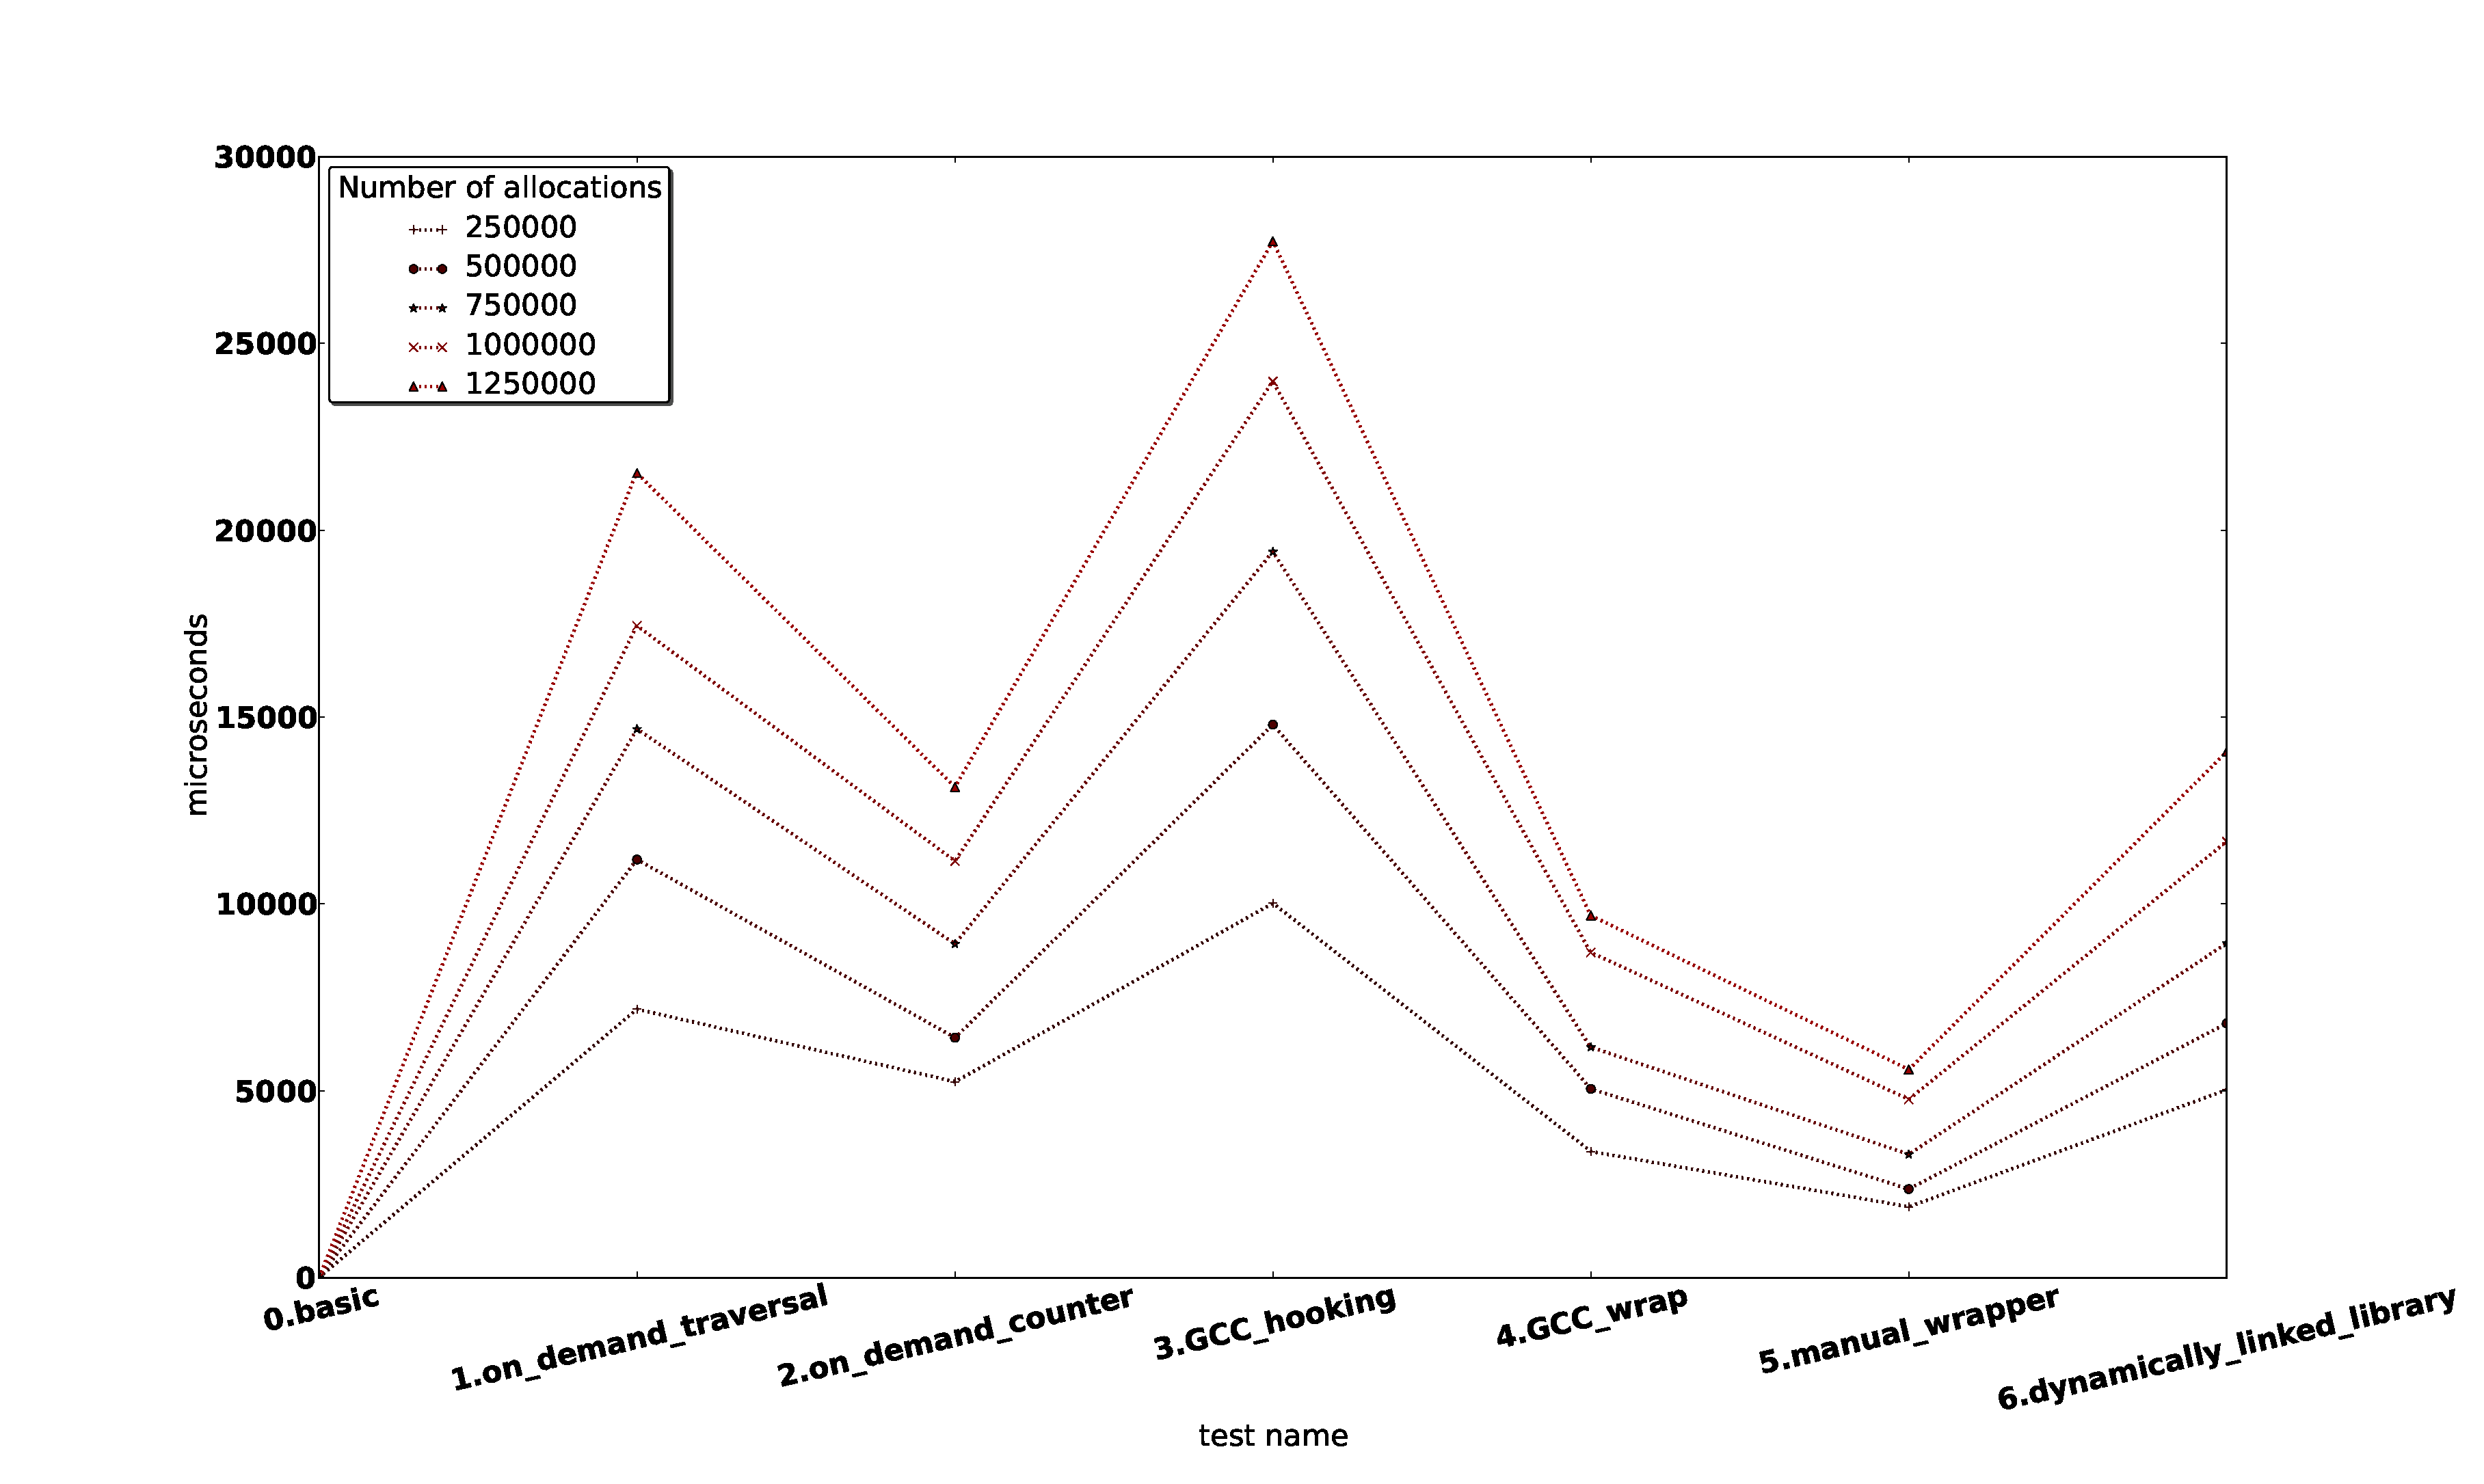
\includegraphics[width=1.0\textwidth]{src/img/allocationsizewithoutlogging}
\caption{Allocation size time overhead compared to the basic scenario when no logging is done}
\label{fig:allocszwithoutlog}
\end{figure}

\begin{figure}[htb]
\centering
\includegraphics[scale=0.5, width=\textwidth]{src/img/allocationsizewithlogging}
\caption{Allocation size time overhead compared to the basic scenario when logging is done}
\label{fig:allocszwithlog}
\end{figure}

In figure \ref{fig:allocszwithoutlog} we can see that the overhead of overloading is lower than the traversal's when we only increment/decrement the global variable. This is explained by the fact that the traversal involves sequential access through each list element which in turn generates extra page faults and cache misses. The overhead of these additional memory accesses is thus higher at this point than the work done inside the overloaded allocation routines. In figure \ref{fig:allocszwithlog} however, we can see that this is no longer true when we add the stack walking. The conclusion to be drawn from this is that the actual mechanisms used to obtain the allocation size information are not the ones inducing the overhead but rather the work performed inside these mechanisms. Since a lot of work needs to be done in the overloaded allocation routines in order to correctly identify the place where the allocation was made, they do perform worse than the traversal techniques.

\section{Allocation point overhead results}
\label{section:allocpt}

In figure \ref{fig:allocpoint} the time overhead of the allocation point determination is shown. While it may seem that the malloc hooks provide the best solution, it has to be mentioned that they only provide the caller of the malloc routine which makes them useless for practical purposes. For the hooks to provide the same amount of information as the other methods, they would have to be augmented with a similar stack walking routine which would put them on the same overhead level as the manual walking method.

Comparing the global stack object with manual stack walking we can see that the former appears to be significantly better. There is one small catch related to the global stack object and that is its behaviour in a multithreaded environment. Multiple buffers are required, one for each thread. Additional code has to be added to check which thread has called the current function, in order to determine in which buffer the trace will be placed. Another disadvantage is that every method has to be augmented at entry and exit points with calls to the object's logging method. This could be done before compile time, by an automatic script. That being said, calls are expensive so inlining might be a solution, at the expense of increased code size.

Finally, using libunwind has such a high overhead that when the results get added to the graph, the other three methods' plot points degenerate into a line. It has thus been omitted from the graph but the method does have its merits. Such a library represents the most portable way of implementing allocation point tracing. Being able to ignore all the low-level details and use a common interface for all of them represents a huge benefit which might make this method suitable if the performance hit is acceptable to the application.

\begin{figure}[htb]
\centering
\includegraphics[scale=0.5, width=\textwidth]{src/img/allocationpoint}
\caption{Allocation point time overhead compared to the basic scenario}
\label{fig:allocpoint}
\end{figure}

All of the above methods have some overhead, so the question is if we can minimize that overhead no matter what method we choose. The first observation we can make is that in the method analysis we have tried to obtain stack traces at each and every allocation the program makes. While this does provide a complete view of an application's memory usage characteristics it is unnecessary for analysis targeting memory spikes and high memory consumption, which is what we are interested in. The typical usage scenario of the profiler we want is the following:

\begin{enumerate}
\item Have a complete view of the memory consumption of different modules in the application
\item Observe one or more modules which show an unusually high memory consumption
\item Trigger more in-depth analysis of those modules by showing the most frequently called allocations done inside the module
\item Enable stack trace logging only for those allocations which are frequently called
\end{enumerate}

By doing the above we can see the call chain which leads to frequent allocations and identify points which can be optimized for better performance.

This is the part where the low-overhead tracepoints come into play. Each allocation routine can have such a tracepoint attached which is disabled by default, by being a noop. The tracepoint, when enabled, does a jump to a routine which either does a simple call count or a full-fledged stack trace, depending on a flag. The enabling of these tracepoints is done entirely on-demand, thus avoiding the overhead of having all the allocation routines do stack trace logging. Combining the tracepoints with any of the allocation point methods above, leads to a lightweight solution that is, however, platform specific and not easily implementable.

\section{Other issues}
\label{section:otherissues}

There are other issues which the tests do not tackle, yet they are important for a complete solution:
\begin{enumerate}
\item \textit{Information storage and analysis} - The test programs use a circular, fixed size buffer for storing the stack traces up to a certain depth. This solution has to be extended to add allocation size information and to allow grouping of stack traces. Two allocations made from the same point have the same stack trace and thus the size should be modified accordingly. Exactly how much of the stack trace is to be compared for equality is another discussion. A shallow comparison of just a couple of stack frames from the trace might not be too useful if the allocations are done in a number of function calls larger than the analysis depth. A specialized allocator might be such an implementation and a shallow analysis would just reveal how the allocator works when in fact we are interested in determining who called the allocator.

Another related problem is where this analysis should be performed. If it is performed at the allocation points we run into the risk of very large overhead. Another approach is to simply add everything into the data structure which holds the traces and let the visualisation component handle the analysis. This way, it gets triggered on-demand and incurs less overhead.

We can also ask ourselves how long should the information be stored? Do we just keep the N most recent stack traces or do we keep all the traces since the program has started? It depends on what type of analysis is done. If we want to be able to track visually the memory consumption and just make sure that everything is in acceptable parameters, a shorter history can be kept. This, however, has the danger of missing memory spikes, where memory consumption increases rapidly but it is not noticed. Here, a longer history is required, to be used by analysis tools and not just for visual inspection. Naturally, the longer the history, the more memory it consumes and writing information to disk very often has a very large time penalty since I/O is inherently slow. A middle ground is required, where the data is dumped periodically on disk or during low activity times.

\item \textit{Concurrency} - Different threads use different stacks and the analysis needs to take this into consideration. Moreover, the data structure holding the traces now needs to be locked to protect it from simultaneous access from multiple threads trying to push stack traces. The visualiser also needs to fetch data from the data structure and thus has to lock it completely to make sure that it is not modified while being read. This scenario can be described as a multiple writers, one reader situation.

\end{enumerate}


\chapter{Conclusion}
\label{chapter:conclusion}

\textbf{And so it ends.}\\



\clearpage
\addcontentsline{toc}{chapter}{Bibliography}
\bibliographystyle{plain}
\bibliography{src/base/references}

\end{document}
